%%% AgriHome — Detailed Design Specification (CSE 4317, Summer 2026)
%%% Structure: AH-109 … AH-116 (Summer DDS template). Content: real implementation.

\documentclass[11pt,letterpaper]{article}
\usepackage[margin=1.0in]{geometry}
\usepackage[T1]{fontenc}
\usepackage[utf8]{inputenc}
\usepackage{array}
\usepackage{booktabs}
\usepackage{longtable}
\usepackage{tabularx}
\usepackage{amssymb}
\usepackage{xcolor}
\usepackage{graphicx}
\usepackage{float}
\usepackage[hidelinks]{hyperref}
\usepackage{fancyhdr}
\usepackage{lastpage}
\usepackage{tikz}
\usetikzlibrary{arrows.meta,positioning,fit,calc}

\graphicspath{{images/}}

\definecolor{accentcolor}{rgb}{0.0,0.0,0.5}
\definecolor{leafgreen}{RGB}{61,159,108}

\newcommand{\teamname}{AgriHome}
\newcommand{\coursename}{CSE 4317: Senior Design II}
\newcommand{\semester}{Summer 2026}
\newcommand{\docname}{Detailed Design Specification}
\newcommand{\department}{Department of Computer Science \& Engineering}
\newcommand{\university}{The University of Texas at Arlington}
\newcommand{\authors}{%
  GOVINDA AWASTHI\\
  LAXMAN BHUSHAL\\
  THUC DANG\\
  SAGAR KHADKA\\
  MUHAMMAD SAAD MEMON\\
  ALEX TABLIZO\\
  NATHAN NGUYEN TRAN}

\pagestyle{fancy}
\lhead{}
\chead{}
\rhead{}
\lfoot{\footnotesize \teamname\ - \semester}
\cfoot{}
\rfoot{\footnotesize page \thepage\ of \pageref{LastPage}}
\renewcommand{\headrulewidth}{0.0pt}
\renewcommand{\footrulewidth}{0.4pt}

\begin{document}

{\centering \huge \color{accentcolor} \scshape \textbf{\department \\ \university} \par}
\vspace{0.65in}
{\centering \huge \color{accentcolor} \scshape \textbf{\docname \\ \coursename \\ \semester} \par}
\vspace{0.4in}
\begin{center}
	
\includegraphics[width=0.52\textwidth]{agrihome-logo}\\[0.55em]
	{\small\slshape AgriHome project logo: leaf and camera lens motif for vision-based agricultural monitoring.}
\end{center}
\vspace{0.45in}
{\centering \huge \color{accentcolor} \scshape \textbf{Team \teamname} \par}
\vspace{0.25in}
{\centering \large \scshape \textbf{\authors} \par}
\newpage

\section*{Revision History}
\begin{center}
\begin{tabular}{@{}llll@{}}
\toprule
\textbf{Revision} & \textbf{Date} & \textbf{Author(s)} & \textbf{Description} \\
\midrule
0.1 & 06.16.2026 & SK, TD & Initial DDS and hardware specification draft \\
0.2 & 06.17.2026 & MSM, AT & Layer-level subsystem designs \\
0.3 & 06.18.2026 & LB, NNT & Template formatting, logo, lists \\
1.0 & 06.18.2026 & GA & Reviewed submission version \\
2.0 & 07.23.2026 & Team & Reflect real Next.js/Postgres/Pi+Moonraker stack \\
2.1 & 07.28.2026 & Team & Klipper edge: fswebcam primary; klipper\_url; updateKlipperUrl \\
\bottomrule
\end{tabular}
\end{center}
\newpage

\tableofcontents
\newpage
\listoffigures
\listoftables
\newpage

%%%%%%%%%%%%%%%%%%%%%%%%%%%%%%%%%%%%%%%%%%%%%%%%%%%%%%%%%%%%%%%%%%%%%%
\section{AH-109: Introduction and System Overview}
%%%%%%%%%%%%%%%%%%%%%%%%%%%%%%%%%%%%%%%%%%%%%%%%%%%%%%%%%%%%%%%%%%%%%%

\subsection{Introduction}
This Detailed Design Specification describes the internal design of \textbf{AgriHome} as
implemented for CSE~4317 Summer~2026. It expands requirements and architecture into
layer-level and subsystem-level designs for the Vision Console, Next.js API routes,
PostgreSQL data model, local file storage, and Raspberry~Pi / Agri-Home/klipper capture path.

Earlier draft wording hypothesized a separate Express backend and fictional tables such as
\texttt{users}, \texttt{images}, \texttt{sensor\_readings}, and \texttt{health\_results}.
\textbf{This revision documents only the live stack:}

\begin{itemize}
  \item \textbf{Frontend:} Next.js App Router Vision Console with \texttt{AppShell}
        (Overview, Trays, Add Plant, Mesh, Feedback, Schedule, \textbf{Devices}, Settings).
  \item \textbf{Backend:} Next.js Route Handlers under \texttt{src/app/api/**} (not Express),
        including \texttt{/api/raspberry-pi/*}, \texttt{/api/devices/*}, trays, plants, camera,
        schedules, files, health, and GraphQL.
  \item \textbf{Database:} PostgreSQL tables \texttt{tray\_systems}, \texttt{plants},
        \texttt{camera\_captures}, \texttt{edge\_devices}, \texttt{edge\_device\_commands},
        \texttt{capture\_pose\_sequences}, \texttt{capture\_poses}, \texttt{capture\_schedules},
        \texttt{prediction\_results}, \texttt{plant\_reports}, \texttt{monitoring\_events}
        (plus mesh/feedback helpers). Base domain tables and edge tables are in
        \texttt{db/schema.sql}; migrations \texttt{009}--\texttt{012} upgrade existing DBs
        (\texttt{011\_capture\_poses.sql} adds pose sequence tables;
        \texttt{012\_klipper\_url.sql} renames \texttt{moonraker\_url} $\rightarrow$ \texttt{klipper\_url}).
  \item \textbf{Storage:} \texttt{STORAGE\_*} originals/processed/temp on the app host,
        served by \texttt{GET /api/files/...}.
  \item \textbf{Hardware:} Raspberry~Pi + Agri-Home/klipper (\texttt{fswebcam} via
        \texttt{camera-macros/save\_image.sh}), optional LAN HTTP streamer for server-side stills,
        and the \texttt{agrihome\_agent} Python
        package; hinge/motor pose fields are modeled (motion may be stubbed).
  \item \textbf{Optional CV:} \texttt{cv-backend} via \texttt{CV\_SPECIES\_INFERENCE\_URL}.
\end{itemize}

\subsection{System Overview}
Operators use the Vision Console. Edge agents register and heartbeat against AgriHome.
Capture is primarily queued (agent runs \texttt{fswebcam} / \texttt{save\_image.sh} and
multipart-ingests); optional immediate path pulls an HTTP streamer still when \texttt{klipper\_url} is set. Domain truth lives in PostgreSQL; binaries live on disk. Optional
inference writes predictions and reports.

\begin{table}[H]
\centering
\begin{tabular}{@{}p{4.2cm}p{9.5cm}@{}}
\toprule
\textbf{Layer} & \textbf{Role} \\
\midrule
Frontend (AH-110) & Vision Console UI for trays, plants, devices, schedules \\
Backend API (AH-111) & Next.js routes + edge/domain services \\
Database (AH-112) & PostgreSQL structured records \\
Storage (AH-113) & Local image files linked by \texttt{camera\_captures.image\_url} \\
Hardware (AH-114) & Pi agent, Klipper/fswebcam, optional pose rig \\
\bottomrule
\end{tabular}
\caption{AgriHome system layers.}
\label{tab:layers}
\end{table}

\begin{figure}[H]
\centering
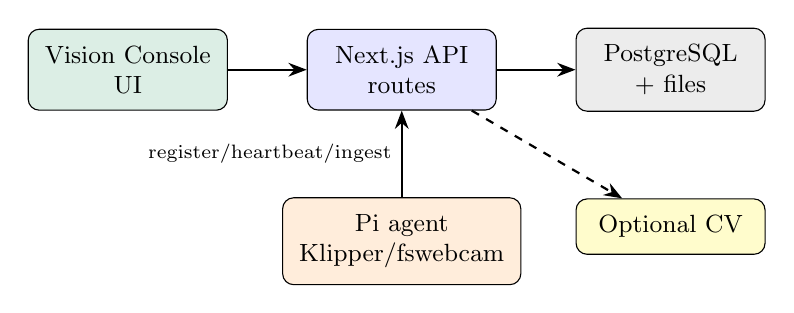
\begin{tikzpicture}[
  font=\small,
  box/.style={draw, rounded corners, align=center, inner sep=6pt, minimum width=2.4cm},
  arr/.style={-{Stealth}, thick}
]
\node[box, fill=leafgreen!18] (ui) {Vision Console\\UI};
\node[box, fill=blue!10, right=1.0cm of ui] (api) {Next.js API\\routes};
\node[box, fill=gray!15, right=1.0cm of api] (pg) {PostgreSQL\\+ files};
\node[box, fill=orange!14, below=1.1cm of api] (pi) {Pi agent\\Klipper/fswebcam};
\node[box, fill=yellow!20, below=1.1cm of pg] (cv) {Optional CV};

\draw[arr] (ui) -- (api);
\draw[arr] (api) -- (pg);
\draw[arr] (pi) -- node[left,font=\scriptsize]{register/heartbeat/ingest} (api);
\draw[arr, dashed] (api) -- (cv);
\end{tikzpicture}
\caption{AgriHome runtime architecture (AH-109 overview).}
\label{fig:dds-overview}
\end{figure}

%%%%%%%%%%%%%%%%%%%%%%%%%%%%%%%%%%%%%%%%%%%%%%%%%%%%%%%%%%%%%%%%%%%%%%
\section{AH-110: Frontend Layer Subsystems}
%%%%%%%%%%%%%%%%%%%%%%%%%%%%%%%%%%%%%%%%%%%%%%%%%%%%%%%%%%%%%%%%%%%%%%

\subsection{Layer Purpose}
Present authenticated operator workflows for monitoring trays and plants, managing schedules
and meshes, viewing captures, and controlling edge devices (Devices page and tray Raspberry~Pi
panel Take Picture).

\subsection{Layer Hardware}
Any modern laptop, desktop, tablet, or phone with a contemporary browser. No client GPU is
required.

\subsection{Layer Operating System}
OS-agnostic browser runtime (macOS, Windows, Linux, iOS/Android browsers). PWA install is
supported where the browser allows.

\subsection{Layer Software Dependencies}
\begin{table}[H]
\centering
\begin{tabular}{@{}p{4.2cm}p{9.5cm}@{}}
\toprule
\textbf{Dependency} & \textbf{Role} \\
\midrule
Next.js App Router / React & Dashboard routes and components \\
TypeScript + Tailwind CSS & Typed UI and styling \\
Firebase client SDK & Operator sign-in \\
Recharts & Health / monitoring charts \\
\texttt{AppShell} + design atoms & Nav shell, FAB, status badges \\
\bottomrule
\end{tabular}
\caption{Frontend layer software dependencies.}
\label{tab:fe-deps}
\end{table}

\subsection{Dashboard Overview Subsystem}
\begin{table}[H]
\centering
\begin{tabular}{@{}p{3.2cm}p{10.5cm}@{}}
\toprule
\textbf{Aspect} & \textbf{Design} \\
\midrule
Route & \texttt{/dashboard} (protected) \\
Purpose & Summarize trays, health, latest frame, and monitoring status \\
Data & Tray list/health snapshot; latest camera frame when available \\
Modules & Server components / tray topology reads; auth gate in protected layout \\
Failure & Empty states when no trays; session redirect when unauthenticated \\
\bottomrule
\end{tabular}
\caption{Dashboard Overview subsystem design details.}
\label{tab:dash}
\end{table}

\subsection{Image Feed Display Subsystem}
Shows latest tray/plant imagery from \texttt{camera\_captures} via \texttt{/api/files/...}
URLs. Tray detail embeds camera panels; plant detail supports photo upload and last-image
display through plant media helpers (\texttt{PlantImage}).

\begin{table}[H]
\centering
\begin{tabular}{@{}p{3.2cm}p{10.5cm}@{}}
\toprule
\textbf{Aspect} & \textbf{Design} \\
\midrule
Purpose & Visual record of current plant / tray condition \\
Source table & \texttt{camera\_captures} (\texttt{image\_url}, \texttt{captured\_at}, pose fields) \\
APIs & \texttt{GET /api/camera/latest}, file bytes via \texttt{GET /api/files/...} \\
UI & Loading/error states; refresh for newest metadata \\
\bottomrule
\end{tabular}
\caption{Image Feed Display subsystem design details.}
\label{tab:image-feed}
\end{table}

\subsection{Plant Health Result UI Subsystem}
Plant and tray pages surface health scores/status, latest diagnosis text, prediction/report
history, and charts. Photo-first add-plant flows call species inference when
\texttt{CV\_SPECIES\_INFERENCE\_URL} is configured. Data comes from \texttt{plants},
\texttt{prediction\_results}, and \texttt{plant\_reports}.

\subsection{Monitoring History Subsystem}
Monitoring events and reports are listed per tray/plant. Historical captures remain browsable
subject to disk retention. Schedule pages show next/last run metadata from
\texttt{capture\_schedules}.

\subsection{Alerts and Notifications UI Subsystem}
In-console alerts appear as \texttt{monitoring\_events} and status badges
(healthy/warning/critical). Device stale marking surfaces offline Pis on the Devices page.
Remote push/email remains future scope.

\subsection{Responsive Navigation and Layout Subsystem}
\texttt{AppShell} provides desktop sidebar and mobile bottom navigation with FAB for Add Plant.
Primary nav: Overview, Trays, Mesh, Feedback (preference-gated), Schedule, and \textbf{Devices}.
Settings is appended. Safe-area padding supports mobile PWA use.

\textbf{TrayEdgeDevicePanel} (tray detail) exposes Take Picture, Klipper/streamer URL edit, device
link, and pose-generation entry points for provisioned Pis.

%%%%%%%%%%%%%%%%%%%%%%%%%%%%%%%%%%%%%%%%%%%%%%%%%%%%%%%%%%%%%%%%%%%%%%
\section{AH-111: Backend API Layer Subsystems}
%%%%%%%%%%%%%%%%%%%%%%%%%%%%%%%%%%%%%%%%%%%%%%%%%%%%%%%%%%%%%%%%%%%%%%

\subsection{Layer Purpose}
Authenticate operators and devices, orchestrate domain services, persist to PostgreSQL/files,
queue edge commands, and optionally call CV inference.

\subsection{Layer Hardware}
Application host (developer laptop, lab server, or container) with network access to PostgreSQL
and, for optional server-side stills, to Pi HTTP streamer URLs stored as \texttt{klipper\_url}.

\subsection{Layer Operating System}
Linux or macOS hosts are typical; Node.js runtime as pinned by the repository.

\subsection{Layer Software Dependencies}
Next.js Route Handlers, \texttt{pg} pool, Firebase Admin/session verification, multipart parsers
for ingest, and HTTP clients for optional streamer stills + CV URLs.

\subsection{Authentication and User Management API}
\begin{itemize}
  \item \texttt{POST /api/auth/session} --- establish server session from Firebase ID token.
  \item \texttt{POST /api/auth/logout} --- clear session cookie.
  \item Protected handlers require verified session email for ownership scoping
        (\texttt{owner\_email}).
\end{itemize}
Device identity is separate: header \texttt{X-Agrihome-Device-Key} on
\texttt{/api/raspberry-pi/*} routes (hashed key in \texttt{edge\_devices}).

\subsection{Plant and Tray Management API}
Representative endpoints: \texttt{GET/POST /api/trays},
\texttt{GET/PATCH /api/trays/\{trayId\}}, \texttt{POST /api/trays/\{trayId\}/vision},
\texttt{GET/POST /api/plants}, \texttt{POST /api/plants/from-photo},
\texttt{POST /api/plants/manual}, \texttt{GET/PATCH/DELETE /api/plants/\{plantId\}},
photo upload, reports, mesh, schedules, monitoring log, preferences, and GraphQL.

\subsection{Image Upload and Retrieval API}
\begin{itemize}
  \item Operator/camera: \texttt{POST /api/camera/ingest}, \texttt{GET /api/camera/latest}.
  \item Edge: \texttt{POST /api/raspberry-pi/ingest} (multipart; device key).
  \item Retrieval: \texttt{GET /api/files/[...path]} for stored originals/processed.
\end{itemize}

\subsection{Edge Device API (replaces draft ``sensor data API'')}
AgriHome does not expose a generic environmental-sensor REST surface in the Summer~2026 cut.
Edge capture is first-class:

\begin{itemize}
  \item \texttt{POST /api/raspberry-pi/register} --- provisioning code + fingerprint $\rightarrow$
        device, one-time API key, linked tray.
  \item \texttt{POST /api/raspberry-pi/heartbeat} --- online status + command claim.
  \item \texttt{GET /api/raspberry-pi/commands}, \texttt{/poses}, \texttt{/capture-plan}.
  \item \texttt{GET /api/devices}, \texttt{GET/POST /api/devices/\{deviceId\}} actions:
        \texttt{capture}, \texttt{linkTray}, \texttt{revoke}, \texttt{rotateKey},
        \texttt{updateKlipperUrl} (alias \texttt{updateMoonrakerUrl}), \texttt{updateLimits}.
  \item \texttt{GET/POST /api/trays/\{trayId\}/poses} --- pose sequences for multi-angle capture.
\end{itemize}

\subsection{Edge Service Mapping (implementation anchors)}
\begin{table}[H]
\centering
\begin{tabular}{@{}p{3.6cm}p{5.0cm}p{5.0cm}@{}}
\toprule
\textbf{Capability} & \textbf{Service module} & \textbf{Primary tables / APIs} \\
\midrule
Edge registration & \texttt{edge-device-service.ts} & \texttt{edge\_devices},
  \texttt{tray\_systems}; \texttt{POST .../register} \\
Heartbeat / stale & \texttt{edge-device-service.ts} & \texttt{edge\_devices.last\_heartbeat\_at};
  \texttt{POST .../heartbeat} \\
Capture commands & \texttt{edge-command-service.ts} & \texttt{edge\_device\_commands};
  claim on heartbeat \\
Ingest storage & \texttt{edge-capture-service.ts},
  camera/storage helpers & files + \texttt{camera\_captures};
  \texttt{POST .../ingest} \\
Plant attach & \texttt{edge-plant-attach-service.ts} & \texttt{plants}, pose slot hints \\
Disease hook & \texttt{edge-disease-hook.ts} & \texttt{prediction\_results} /
  \texttt{plant\_reports}, \texttt{monitoring\_events} \\
Vision hook & \texttt{edge-vision-hook.ts} & optional auto vision after ingest \\
Postprocess & \texttt{edge-capture-postprocess.ts} & attach + optional hooks after save \\
\bottomrule
\end{tabular}
\caption{Edge capabilities mapped to real modules and tables.}
\label{tab:edge-map}
\end{table}

\subsection{Plant Health Analysis API}
Predictions via \texttt{GET /api/predictions/latest} and service-layer calls to
\texttt{CV\_SPECIES\_INFERENCE\_URL} / tray vision. Optional auto vision after Pi ingest when
\texttt{DEVICE\_AUTO\_VISION\_ON\_INGEST} is enabled.

\subsection{Alerts API}
Monitoring events are created/read through monitoring services and
\texttt{/api/monitoring/log}. Device stale marking runs when listing devices. Dedicated push
notification API remains future.

%%%%%%%%%%%%%%%%%%%%%%%%%%%%%%%%%%%%%%%%%%%%%%%%%%%%%%%%%%%%%%%%%%%%%%
\section{AH-112: Database / Data Layer Subsystems}
%%%%%%%%%%%%%%%%%%%%%%%%%%%%%%%%%%%%%%%%%%%%%%%%%%%%%%%%%%%%%%%%%%%%%%

\subsection{Layer Purpose}
Provide durable relational storage for AgriHome domain entities and edge lifecycle state.

\subsection{Layer Hardware}
PostgreSQL server (local Docker, lab VM, or managed instance).

\subsection{Layer Operating System}
PostgreSQL-supported OS; accessed over TCP from the Next.js host.

\subsection{Layer Software Dependencies}
PostgreSQL~14+ recommended; SQL under \texttt{db/schema.sql} and
\texttt{db/migrations/} (\texttt{009\_edge\_devices.sql},
\texttt{010\_camera\_ingest\_metadata.sql}, \texttt{011\_capture\_poses.sql}).

\subsection{Database Schema Summary}
The live schema does \textbf{not} use fictional \texttt{users}, \texttt{images},
\texttt{sensor\_readings}, or \texttt{health\_results} tables. Firebase identifies humans;
PostgreSQL stores domain rows keyed largely by \texttt{owner\_email} and string IDs.

\begin{table}[H]
\centering
\begin{tabular}{@{}llp{7.2cm}@{}}
\toprule
\textbf{Table} & \textbf{Migration} & \textbf{Role} \\
\midrule
\texttt{tray\_systems} & base / 009 & Tray metadata, health, optional \texttt{edge\_device\_id} \\
\texttt{plants} & base & Plants in trays; slot/row/column; diagnosis fields \\
\texttt{camera\_captures} & base / 010 & Capture metadata + image URL + pose fields \\
\texttt{edge\_devices} & 009+012 & Pi identity, key hash, \texttt{klipper\_url}, heartbeat \\
\texttt{edge\_device\_commands} & 009 & Pending/claimed/completed device commands \\
\texttt{capture\_pose\_sequences} & 011 & Active pose sequences per tray \\
\texttt{capture\_poses} & 011 & Ordered hinge/motor/dwell poses \\
\texttt{capture\_schedules} & base & Interval schedules; destination may be
  \texttt{raspberry-pi-edge} \\
\texttt{prediction\_results} & base & Classifier outputs linked to captures \\
\texttt{plant\_reports} & base & Structured diagnosis reports \\
\texttt{monitoring\_events} & base & Alert/log stream \\
\texttt{mesh\_networks} & base & Tray groupings \\
\texttt{feedback\_ingest} / \texttt{user\_preferences} & base & ML feedback opt-in \& samples \\
\bottomrule
\end{tabular}
\caption{Actual PostgreSQL tables used by AgriHome.}
\label{tab:schema-summary}
\end{table}

\subsection{\texttt{tray\_systems} Table}
Primary key \texttt{id}; \texttt{owner\_email}, \texttt{name}, \texttt{zone}, \texttt{crop},
counts, health/status, \texttt{device\_id}, nullable \texttt{edge\_device\_id},
\texttt{last\_capture\_at}, timestamps/vision summary fields.

\subsection{\texttt{plants} Table}
Primary key \texttt{id}; \texttt{tray\_id} FK; mesh IDs JSON; name/cultivar/slot/indices;
health; \texttt{latest\_diagnosis}; optional description;
\texttt{last\_image\_url}/\texttt{last\_image\_at}.

\subsection{\texttt{camera\_captures} Table}
Replaces fictional \texttt{images}. Stores \texttt{image\_url}, \texttt{captured\_at},
\texttt{source}, \texttt{status}, optional \texttt{plant\_id}, \texttt{hinge\_deg},
\texttt{motor\_mm}, \texttt{pose\_order}, \texttt{command\_id} (migration~010).

\subsection{\texttt{edge\_devices} Table}
\texttt{cpu\_serial} unique; \texttt{api\_key\_hash} + \texttt{api\_key\_prefix};
\texttt{klipper\_url}; \texttt{status}; \texttt{last\_heartbeat\_at}; hinge/motor range
fields; \texttt{revoked\_at}.

\subsection{\texttt{edge\_device\_commands} Table}
Command queue: \texttt{command\_type} (e.g.\ \texttt{capture\_now}, \texttt{sync\_poses},
\texttt{reboot\_agent}), \texttt{payload\_json}, \texttt{status}, claim/complete timestamps,
optional result/error.

\subsection{\texttt{capture\_pose\_sequences} / \texttt{capture\_poses}}
Multi-angle capture plans for trays/devices (AGRI-104). Poses include hinge degrees, motor mm,
dwell, optional plant/slot binding.

\subsection{\texttt{capture\_schedules} Table}
\texttt{interval\_minutes}, \texttt{next\_run\_at}, \texttt{destination} defaulting to
\texttt{computer-vision-backend} or set to \texttt{raspberry-pi-edge}.

\subsection{\texttt{prediction\_results} / \texttt{plant\_reports} / \texttt{monitoring\_events}}
Persist CV outputs, structured reports (diseases/deficiencies JSON), and operator-visible
events. These supersede earlier draft \texttt{health\_results}/\texttt{alerts}/
\texttt{monitoring\_history} names.

\subsection{Indexing, Retention, and Validation Strategy}
Indexes exist on owner emails, edge status, pending commands, tray/plant captures, and pose
ordering. Application services validate ownership and foreign keys. Image retention is
operational (disk capacity); no automatic cold-archive job is mandated in the prototype.

%%%%%%%%%%%%%%%%%%%%%%%%%%%%%%%%%%%%%%%%%%%%%%%%%%%%%%%%%%%%%%%%%%%%%%
\section{AH-113: Storage File Management Systems}
%%%%%%%%%%%%%%%%%%%%%%%%%%%%%%%%%%%%%%%%%%%%%%%%%%%%%%%%%%%%%%%%%%%%%%

\subsection{Layer Purpose}
Persist binary imagery referenced by relational rows without forcing blobs into git or a single
cloud vendor during development. Files live on the \textbf{application host} (not on a
per-user Pi SSD as an earlier draft suggested).

\subsection{Layer Hardware}
Local disk or mounted volume on the Next.js host.

\subsection{Layer Operating System}
Host filesystem semantics (POSIX typical).

\subsection{Layer Software Dependencies}
\texttt{STORAGE\_ROOT}, \texttt{STORAGE\_ORIGINALS\_DIR}, \texttt{STORAGE\_PROCESSED\_DIR},
\texttt{STORAGE\_TEMP\_DIR} resolution helpers; Next.js file route;
\texttt{save-original} / leaf storage helpers used by edge ingest.

\subsection{File Management Subsystems}
\begin{table}[H]
\centering
\begin{tabular}{@{}p{4.5cm}p{9.2cm}@{}}
\toprule
\textbf{Subsystem} & \textbf{Processing} \\
\midrule
Image Upload & Validate type/size; write original; insert \texttt{camera\_captures} \\
Folder organization & Generated names under originals/processed/temp trees \\
Image Retrieval & \texttt{GET /api/files/[...path]} streams allowlisted bytes \\
Cleanup / Archiving & Manual/ops for prototype; future cold archive optional \\
Security & Session for operator uploads; device key for Pi ingest \\
\bottomrule
\end{tabular}
\caption{Storage subsystem summary.}
\label{tab:storage}
\end{table}

\subsection{Image Upload Subsystem}
Accepts operator uploads and device multipart ingest; writes files then inserts
\texttt{camera\_captures} with a stable \texttt{/api/files/...} URL.

\subsection{File Naming and Folder Organization Subsystem}
Opaque/generated filenames under logical folders as implemented by storage helpers; keys stored
in DB rather than user-supplied paths.

\subsection{Image Retrieval Subsystem}
\texttt{GET /api/files/[...path]} streams bytes for Console \texttt{next/image} / media
components with local pattern allowlisting.

\subsection{Image Cleanup and Archiving Subsystem}
Manual/ops cleanup for the prototype; future archive jobs may move cold originals off primary
disk.

\subsection{Security and Access Control Subsystem}
File routes are application-mediated. Device ingest requires device API key. Operator uploads
require session auth. Host OS permissions must protect \texttt{STORAGE\_*} directories.

%%%%%%%%%%%%%%%%%%%%%%%%%%%%%%%%%%%%%%%%%%%%%%%%%%%%%%%%%%%%%%%%%%%%%%
\section{AH-114: Hardware / Camera Layer Subsystems}
%%%%%%%%%%%%%%%%%%%%%%%%%%%%%%%%%%%%%%%%%%%%%%%%%%%%%%%%%%%%%%%%%%%%%%

\subsection{Layer Purpose}
Capture tray imagery on the bench and deliver it to AgriHome with minimal operator toil.

\subsection{Layer Hardware}
\begin{itemize}
  \item Raspberry~Pi (or compatible) running Agri-Home/klipper with \texttt{fswebcam}.
  \item Primary stills via \texttt{camera-macros/save\_image.sh}; optional HTTP streamer
        stills (e.g.\ \texttt{/webcam/?action=snapshot} on nginx \texttt{:80}) when
        \texttt{klipper\_url} is configured for server-side Take Picture.
  \item Optional hinge/motor rig for multi-pose capture (fields modeled; motion may be stubbed).
  \item Plant tray/rack fixture and lighting as built in makerspaces.
\end{itemize}

\begin{table}[H]
\centering
\begin{tabular}{@{}p{4.2cm}p{9.5cm}@{}}
\toprule
\textbf{Component} & \textbf{Role} \\
\midrule
Raspberry Pi & Runs \texttt{agrihome\_agent} + Agri-Home/klipper \\
Klipper / fswebcam & Primary JPEG source via \texttt{save\_image.sh} \\
AgriHome agent & Register, heartbeat, claim commands, multipart ingest \\
Vision Console & Operator Take Picture / Devices / Klipper URL edit \\
\bottomrule
\end{tabular}
\caption{Hardware prototype component summary.}
\label{tab:hw}
\end{table}

\subsection{Layer Operating System}
Raspberry Pi OS (or similar Linux) with Python~3 for \texttt{agrihome\_agent}.

\subsection{Layer Software Dependencies}
Agri-Home/klipper, \texttt{fswebcam}, \texttt{agrihome\_agent} (register/run) from the
Agri-Home/moonraker companion repo (\texttt{feature/agrihome-bridge}; configured for
\texttt{klipperUrl} + fswebcam), network access to AgriHome base URL, shared
\texttt{DEVICE\_PROVISIONING\_SECRET}. Ops detail:
\texttt{docs/ops/RASPBERRY\_PI\_KLIPPER.md}.

\subsection{Camera Capture Subsystem}
Two paths:
\begin{enumerate}
  \item \textbf{Primary --- agent + fswebcam:} command \texttt{capture\_now} claimed on
        heartbeat; agent runs Agri-Home/klipper \texttt{camera-macros/save\_image.sh} and
        \texttt{POST}s multipart ingest.
  \item \textbf{Optional --- HTTP streamer still:} when \texttt{klipper\_url} is set and
        reachable, AgriHome may fetch still candidates (common \texttt{:80} webcam paths)
        via \texttt{captureFromKlipperStreamerDirect} in \texttt{edge-capture-service.ts}
        before queuing the agent.
\end{enumerate}

\subsection{Plant Rack Positioning Subsystem}
Pose sequences define hinge degrees and motor millimeters per plant slot. Agent walks poses when
\texttt{runPoses} is set; failed poses should not abort the entire sequence. Physical motion
drivers may be stubs pending hardware bring-up. Tables:
\texttt{capture\_pose\_sequences}, \texttt{capture\_poses}.

\subsection{Device Communication Subsystem}
Agent $\leftrightarrow$ AgriHome over HTTP(S): register, heartbeat, commands, poses,
capture-plan, ingest. Console $\leftrightarrow$ AgriHome for device actions. AgriHome
$\leftrightarrow$ optional HTTP streamer for direct stills.

\subsection{Power and Reliability Subsystem}
USB/wall power for Pi and lighting; heartbeat stale window
(\texttt{DEVICE\_HEARTBEAT\_STALE\_MINUTES}) marks offline devices; revoke/re-provision recovers
credentials after compromise or replacement.

\subsection{Hardware Layer Limitations}
\begin{itemize}
  \item Server-side snapshot requires AgriHome host reachability to the Pi (LAN/WARP caveats).
  \item Optional streamer URL paths vary by nginx/mjpegstreamer configuration.
  \item No autonomous plant-care actuation (watering/dosing) in scope.
  \item Environmental sensors remain optional relative to webcam capture.
\end{itemize}

%%%%%%%%%%%%%%%%%%%%%%%%%%%%%%%%%%%%%%%%%%%%%%%%%%%%%%%%%%%%%%%%%%%%%%
\section{AH-115: System Overview and Architecture Diagram}
%%%%%%%%%%%%%%%%%%%%%%%%%%%%%%%%%%%%%%%%%%%%%%%%%%%%%%%%%%%%%%%%%%%%%%

\subsection{Architecture Explanation}
AgriHome is a layered web application with an edge capture extension. The UI never talks to
PostgreSQL directly. Device credentials are not Firebase users. CV is an optional processing
adapter.

\subsection{Architecture Diagram}
\begin{figure}[H]
\centering
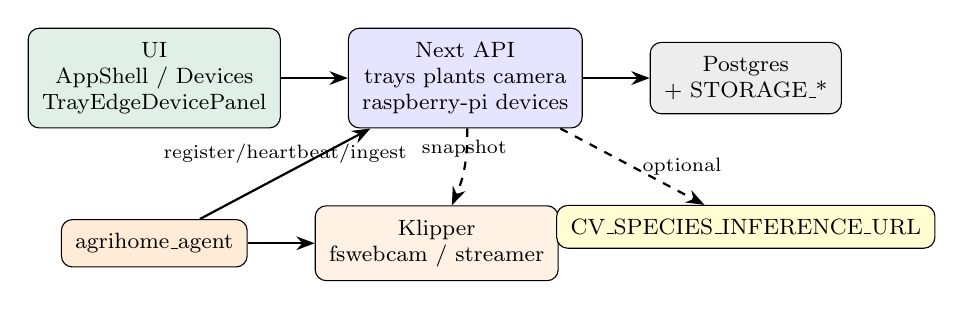
\begin{tikzpicture}[
  font=\footnotesize,
  box/.style={draw, rounded corners, align=center, inner sep=5pt},
  arr/.style={-{Stealth}, thick}
]
\node[box, fill=leafgreen!16] (ui) {UI\\AppShell / Devices\\TrayEdgeDevicePanel};
\node[box, fill=blue!10, right=0.85cm of ui] (api) {Next API\\trays plants camera\\raspberry-pi devices};
\node[box, fill=gray!14, right=0.85cm of api] (data) {Postgres\\+ STORAGE\_*};
\node[box, fill=orange!16, below=1.15cm of ui] (agent) {agrihome\_agent};
\node[box, fill=orange!10, right=0.85cm of agent] (mr) {Klipper\\fswebcam / streamer};
\node[box, fill=yellow!18, below=1.15cm of data] (cv) {CV\_SPECIES\_INFERENCE\_URL};

\draw[arr] (ui) -- (api);
\draw[arr] (api) -- (data);
\draw[arr] (agent) -- node[above,font=\scriptsize]{register/heartbeat/ingest} (api);
\draw[arr] (agent) -- (mr);
\draw[arr, dashed] (api) -- node[right,font=\scriptsize]{optional} (cv);
\draw[arr, dashed] (api) to[bend left=12] node[above,font=\scriptsize]{snapshot} (mr);
\end{tikzpicture}
\caption{UI $\leftrightarrow$ Next API $\leftrightarrow$ Postgres/files; Pi agent
$\leftrightarrow$ register/heartbeat/ingest; optional CV.}
\label{fig:dds-arch}
\end{figure}

\noindent\textit{Mermaid equivalent (documentation form):}
\begin{verbatim}
flowchart LR
  UI[Vision Console] --> API[Next.js API]
  API --> DB[(PostgreSQL)]
  API --> FS[STORAGE_* files]
  Agent[agrihome_agent] -->|register/heartbeat/ingest| API
  Agent --> MR[Klipper fswebcam]
  API -.->|optional snapshot| MR
  API -.->|CV_SPECIES_INFERENCE_URL| CV[cv-backend]
\end{verbatim}

\subsection{Architecture Data Flow}
\begin{enumerate}
  \item Agent registers $\rightarrow$ \texttt{edge\_devices} + tray + one-time API key.
  \item Heartbeat loop updates presence and claims commands from
        \texttt{edge\_device\_commands}.
  \item Operator Take Picture $\rightarrow$ queued \texttt{capture\_now} (fswebcam) or
        optional streamer still $\rightarrow$ file + \texttt{camera\_captures} row;
        plant attach via \texttt{edge-plant-attach-service}.
  \item Optional disease/vision hooks $\rightarrow$ \texttt{prediction\_results} /
        \texttt{plant\_reports} + \texttt{monitoring\_events}.
  \item Console reads trays/plants/devices/captures for display.
\end{enumerate}

\subsection{Interface Summary}
\begin{center}
\begin{longtable}{@{}llp{5.8cm}@{}}
\toprule
\textbf{Method} & \textbf{Path} & \textbf{Auth / Purpose} \\
\midrule
\endfirsthead
\toprule
\textbf{Method} & \textbf{Path} & \textbf{Auth / Purpose} \\
\midrule
\endhead
POST & \texttt{/api/raspberry-pi/register} & Provisioning secret; create device+tray \\
POST & \texttt{/api/raspberry-pi/heartbeat} & Device key; presence + claim commands \\
POST & \texttt{/api/raspberry-pi/ingest} & Device key; multipart image upload \\
GET & \texttt{/api/raspberry-pi/commands} & Device key; pending commands \\
GET & \texttt{/api/raspberry-pi/poses} & Device key; active pose sequence \\
GET & \texttt{/api/raspberry-pi/capture-plan} & Device key; schedules+poses+limits \\
GET & \texttt{/api/devices} & Session; list devices \\
POST & \texttt{/api/devices/\{id\}} & Session; capture/link/revoke/rotate/URL \\
GET/POST & \texttt{/api/trays/\{id\}/poses} & Session; configure poses \\
GET/POST & \texttt{/api/trays}, \texttt{/api/plants} & Session; tray/plant CRUD \\
GET & \texttt{/api/files/...} & App-mediated file bytes \\
GET & \texttt{/api/health} & DB + inference configuration probe \\
\bottomrule
\caption{Backend API endpoint summary (selected real interfaces).}
\label{tab:interfaces}
\end{longtable}
\end{center}

\subsection{Design Rationale}
Reusing Agri-Home/klipper camera macros (\texttt{fswebcam}) avoids a custom camera daemon.
Next.js Route Handlers keep one deployable unit for UI+API. Hashed device keys and a rotatable
provisioning secret match the bench threat model without inventing a second human identity
system in PostgreSQL.

\subsection{Current Implementation Connection}
Source anchors: \texttt{src/app/api/raspberry-pi/*}, \texttt{src/app/api/devices/*},
\texttt{src/lib/services/edge-*.ts}, \texttt{TrayEdgeDevicePanel.tsx}, \texttt{db/schema.sql},
migrations \texttt{009}--\texttt{012}, and ops docs for Pi/Klipper and edge security.

%%%%%%%%%%%%%%%%%%%%%%%%%%%%%%%%%%%%%%%%%%%%%%%%%%%%%%%%%%%%%%%%%%%%%%
\section{AH-116: Final Review and Submit}
%%%%%%%%%%%%%%%%%%%%%%%%%%%%%%%%%%%%%%%%%%%%%%%%%%%%%%%%%%%%%%%%%%%%%%

\subsection{Final Review Checklist}
\begin{itemize}
  \item[$\square$] Cover, roster, revision 2.1 (07.28.2026), Summer 2026 footer present.
  \item[$\square$] AH-109--AH-116 sections complete with real schema/endpoints.
  \item[$\square$] Frontend includes Devices nav and Take Picture panel behavior.
  \item[$\square$] Backend documented as Next.js API routes (not Express).
  \item[$\square$] Hardware section covers Pi + Klipper/fswebcam + agent + optional streamer.
  \item[$\square$] Interface table matches implemented raspberry-pi/devices routes.
  \item[$\square$] Edge services mapped: registration, heartbeat, commands, ingest, plant
        attach, disease hook.
  \item[$\square$] Cross-check with SRS requirements and Charter milestones.
\end{itemize}

\subsection{Revision History Table}
See front-matter revision history (includes 2.1 / 07.28.2026 Klipper edge update).

\subsection{List of Figures / Tables}
Generated automatically by \texttt{\textbackslash listoffigures} and
\texttt{\textbackslash listoftables} in this document's front matter.

\subsection{Appendix Suggestions}
Attach agent README excerpts, example \texttt{agent.json}, sample register/ingest curls, and
Optional streamer URL discovery notes and \texttt{save\_image.sh} smoke-test output.

\section{Appendix A: Suggested Supporting Material}
\begin{itemize}
  \item Ops: \texttt{docs/ops/RASPBERRY\_PI\_KLIPPER.md} (Moonraker stub superseded).
  \item Ops: Edge device security (AGRI-109) controls checklist.
  \item Implementation guide sections for storage and CV env vars.
  \item Physical E2E checklist: migrate, provision, heartbeat online, Take Picture, optional
        poses/schedules.
\end{itemize}

\section{Appendix B: Subsystem $\rightarrow$ Module / Table Map}
\begin{center}
\begin{longtable}{@{}p{3.4cm}p{5.4cm}p{5.0cm}@{}}
\toprule
\textbf{DDS subsystem} & \textbf{Code / routes} & \textbf{Tables} \\
\midrule
\endfirsthead
\toprule
\textbf{DDS subsystem} & \textbf{Code / routes} & \textbf{Tables} \\
\midrule
\endhead
Dashboard / nav & \texttt{AppShell}, dashboard routes & \texttt{tray\_systems},
  \texttt{monitoring\_events} \\
Image feed & camera UI, \texttt{/api/files}, \texttt{/api/camera/*} &
  \texttt{camera\_captures} \\
Plant health UI & plant/tray pages, predictions APIs & \texttt{plants},
  \texttt{prediction\_results}, \texttt{plant\_reports} \\
Edge registration & \texttt{edge-device-service},
  \texttt{/api/raspberry-pi/register} & \texttt{edge\_devices},
  \texttt{tray\_systems} \\
Heartbeat & \texttt{updateDeviceHeartbeat},
  \texttt{/api/raspberry-pi/heartbeat} & \texttt{edge\_devices} \\
Capture commands & \texttt{edge-command-service},
  Devices \texttt{action=capture} & \texttt{edge\_device\_commands} \\
Ingest / snapshot & \texttt{edge-capture-service},
  \texttt{/api/raspberry-pi/ingest} & \texttt{camera\_captures} + files \\
Plant attach & \texttt{edge-plant-attach-service} & \texttt{plants},
  \texttt{capture\_poses} \\
Disease hook & \texttt{edge-disease-hook} & \texttt{prediction\_results},
  \texttt{plant\_reports}, \texttt{monitoring\_events} \\
Poses & \texttt{capture-pose-service}, trays/poses APIs &
  \texttt{capture\_pose\_sequences}, \texttt{capture\_poses} \\
Schedules & schedule APIs / capture-plan & \texttt{capture\_schedules} \\
\bottomrule
\caption{DDS subsystems mapped to real modules and tables.}
\label{tab:subsystem-map}
\end{longtable}
\end{center}

\newpage
\begin{thebibliography}{9}
\bibitem{srs}
AgriHome, \textit{System Requirements Specification}, updated Summer~2026.

\bibitem{ads}
AgriHome, \textit{Architectural Design Specification}, CSE~4316, Spring~2026.

\bibitem{charter}
AgriHome, \textit{Project Charter}, updated Summer~2026.

\bibitem{nextjs}
Vercel, Inc., ``Next.js Documentation,'' \url{https://nextjs.org/docs}.

\bibitem{postgres}
PostgreSQL Global Development Group, ``PostgreSQL Documentation,''
\url{https://www.postgresql.org/docs/}.

\bibitem{firebase}
Google, ``Firebase Authentication,'' \url{https://firebase.google.com/docs/auth}.

\bibitem{klipper}
Agri-Home/klipper companion firmware and \texttt{camera-macros/save\_image.sh};
AgriHome ops guide \texttt{docs/ops/RASPBERRY\_PI\_KLIPPER.md}.
\end{thebibliography}

\end{document}
